\documentclass[11pt,article,oneside]{memoir}
\usepackage{org-preamble-pdflatex}

\usepackage{calc,array}

\usepackage{longtable}

\usepackage{graphicx}
% Redefine \includegraphics so that, unless explicit options are
% given, the image width will not exceed the width or the height of the page.
% Images get their normal width if they fit onto the page, but
% are scaled down if they would overflow the margins.
\makeatletter
\def\ScaleWidthIfNeeded{%
 \ifdim\Gin@nat@width>\linewidth
    \linewidth
  \else
    \Gin@nat@width
  \fi
}
\def\ScaleHeightIfNeeded{%
  \ifdim\Gin@nat@height>0.9\textheight
    0.9\textheight
  \else
    \Gin@nat@width
  \fi
}
\makeatother

\setkeys{Gin}{width=\ScaleWidthIfNeeded,height=\ScaleHeightIfNeeded,keepaspectratio}%


\newlength{\cslhangindent}
\setlength{\cslhangindent}{1.5em}
\newlength{\csllabelwidth}
\setlength{\csllabelwidth}{3em}
\newlength{\cslentryspacingunit} % times entry-spacing
\setlength{\cslentryspacingunit}{\parskip}
\newenvironment{CSLReferences}[2] % #1 hanging-ident, #2 entry spacing
 {% don't indent paragraphs
  \setlength{\parindent}{0pt}
  % turn on hanging indent if param 1 is 1
  \ifodd #1
  \let\oldpar\par
  \def\par{\hangindent=\cslhangindent\oldpar}
  \fi
  % set entry spacing
  \setlength{\parskip}{#2\cslentryspacingunit}
 }%
 {}
\usepackage{calc}
\newcommand{\CSLBlock}[1]{#1\hfill\break}
\newcommand{\CSLLeftMargin}[1]{\parbox[t]{\csllabelwidth}{#1}}
\newcommand{\CSLRightInline}[1]{\parbox[t]{\linewidth - \csllabelwidth}{#1}\break}
\newcommand{\CSLIndent}[1]{\hspace{\cslhangindent}#1}

\title{\bigskip \bigskip The Implications of the War of the Roses on
Anglo-Franco Relations\thanks{Thank you to the everyone that supported
this work.}  }
 

%\author{true\\true}

\author{\Large Timothy
Elder\vspace{0.05in} \newline\normalsize\emph{University of
Chicago} \newline\footnotesize \texttt{\href{mailto:timothyelder@uchicago.edu}{timothyelder@uchicago.edu}}\vspace*{0.2in}\newline  \and \Large Joe
Bloggs\vspace{0.05in} \newline\normalsize\emph{Northwestern
University} \newline\footnotesize \texttt{\href{mailto:joebloggs@northwestern.edu}{joebloggs@northwestern.edu}}\vspace*{0.2in}\newline }

\date{}


\begin{document}  
\setkeys{Gin}{width=1\textwidth} 	
%\setromanfont[Mapping=tex-text,Numbers=OldStyle]{Minion Pro}
%\setsansfont[Mapping=tex-text]{Minion Pro} 
%\setmonofont[Mapping=tex-text,Scale=0.8]{Pragmata}
\chapterstyle{article-4} 
\pagestyle{kjh}

\published{January 2023.}

\maketitle



\begin{abstract}

\vspace*{-0.75in}\noindent \emph{Abstract:} The War of the Roses was a
significant event in English history that had far-reaching implications
for the relationships between England and France. This paper explores
the impact of the conflict on the political, economic, and cultural ties
between the two countries. The war resulted in significant changes to
the English monarchy, which had repercussions for the English crown's
relationships with other European powers, including France. This paper
provides an in-depth analysis of these impacts, and sheds light on the
lasting effects of this important event in English history.

\end{abstract}


\hypertarget{the-war-of-the-roses}{%
\section{The War of the Roses}\label{the-war-of-the-roses}}

The War of the Roses was a series of civil wars fought in England from
1455 to 1487 between the House of Lancaster (represented by a red rose)
and the House of York (represented by a white rose). The conflict was
primarily driven by political and financial power struggles, and
involved several changes of the English monarchy (Bennett 1998).

The wars ended with the victory of the Lancastrian Henry VII, who became
the first monarch of the Tudor dynasty. He united the two houses by
marrying Elizabeth of York, daughter of Edward IV of York, thereby
symbolically uniting the red and white roses (Carpenter 1997).

The War of the Roses had far-reaching impacts on English society and
government. It weakened the power of the nobility and strengthened the
power of the monarchy, setting the stage for the development of the
Tudor state. It also contributed to the decline of feudalism and the
rise of nationalism in England. The conflict is often remembered for the
dramatic and brutal battles that were fought, as well as for its role in
shaping the future of England (Chrimes 1999). Check Figure
\ref{fig:example_fig} for information about this.

\hypertarget{the-plantagenants}{%
\subsection{The Plantagenants}\label{the-plantagenants}}

The Plantagenets were a royal dynasty that ruled England from 1154 to
1485. The dynasty was founded by Henry II, who became king of England
after the death of King Stephen. The Plantagenets were descendants of
the counts of Anjou, in what is now France, and they expanded their
power through a combination of military conquests and political
marriages.

During the Plantagenet era, England experienced significant growth and
expansion. The Plantagenet kings were involved in the Crusades, the
Hundred Years' War with France, and the formation of the British Empire.
They also established many important institutions and laws that shaped
the development of England and the wider world.

The Plantagenets were divided into two branches: the House of Lancaster
and the House of York. These two houses were in conflict during the Wars
of the Roses, a series of civil wars fought from 1455 to 1487. The
conflict ended with the victory of the Lancastrian Henry VII, who became
the first Tudor king of England and united the two houses through his
marriage to Elizabeth of York.

The Plantagenets left a lasting legacy on England and the wider world.
They established the legal and political systems that formed the basis
of modern England, and their rule marked a turning point in English
history, setting the stage for the Renaissance and the development of
modern Europe.

\hypertarget{house-of-lancaster}{%
\subsection{House of Lancaster}\label{house-of-lancaster}}

The House of Lancaster was a royal house of the Kingdom of England,
which ruled from 1399 to 1461, and again from 1470 to 1471. It was the
fourth of the five royal houses of the Plantagenet dynasty to rule
England, and was founded by John of Gaunt, the third son of King Edward
III.

The first Lancaster king was Henry IV, who took the throne in 1399 after
overthrowing his cousin, Richard II. Henry IV's reign was marked by
political turmoil, including rebellion and assassination attempts. His
son, Henry V, became one of England's most successful kings, winning
several major battles in the Hundred Years' War against France.

The House of Lancaster suffered a significant setback in the Wars of the
Roses, a series of civil wars fought between the House of Lancaster and
the House of York from 1455 to 1487. After a series of losses, the
Lancaster dynasty was temporarily overthrown in 1461 by the Yorkist
Edward IV. The Lancaster king, Henry VI, was restored to the throne in
1470, but was soon overthrown again in 1471 by Edward IV.

The last Lancaster king, Henry VI, was a weak ruler who suffered from
mental illness. His rule was marked by political instability, and he was
eventually deposed by the Yorkist Edward IV. The Lancaster dynasty was
succeeded by the Tudor dynasty, which was established by Henry VII, who
defeated the Yorkist Richard III at the Battle of Bosworth Field in
1485. The Tudor dynasty united the houses of Lancaster and York through
the marriage of Henry VII to Elizabeth of York, daughter of Edward IV.

\begin{figure}
\hypertarget{fig:example_fig}{%
\centering
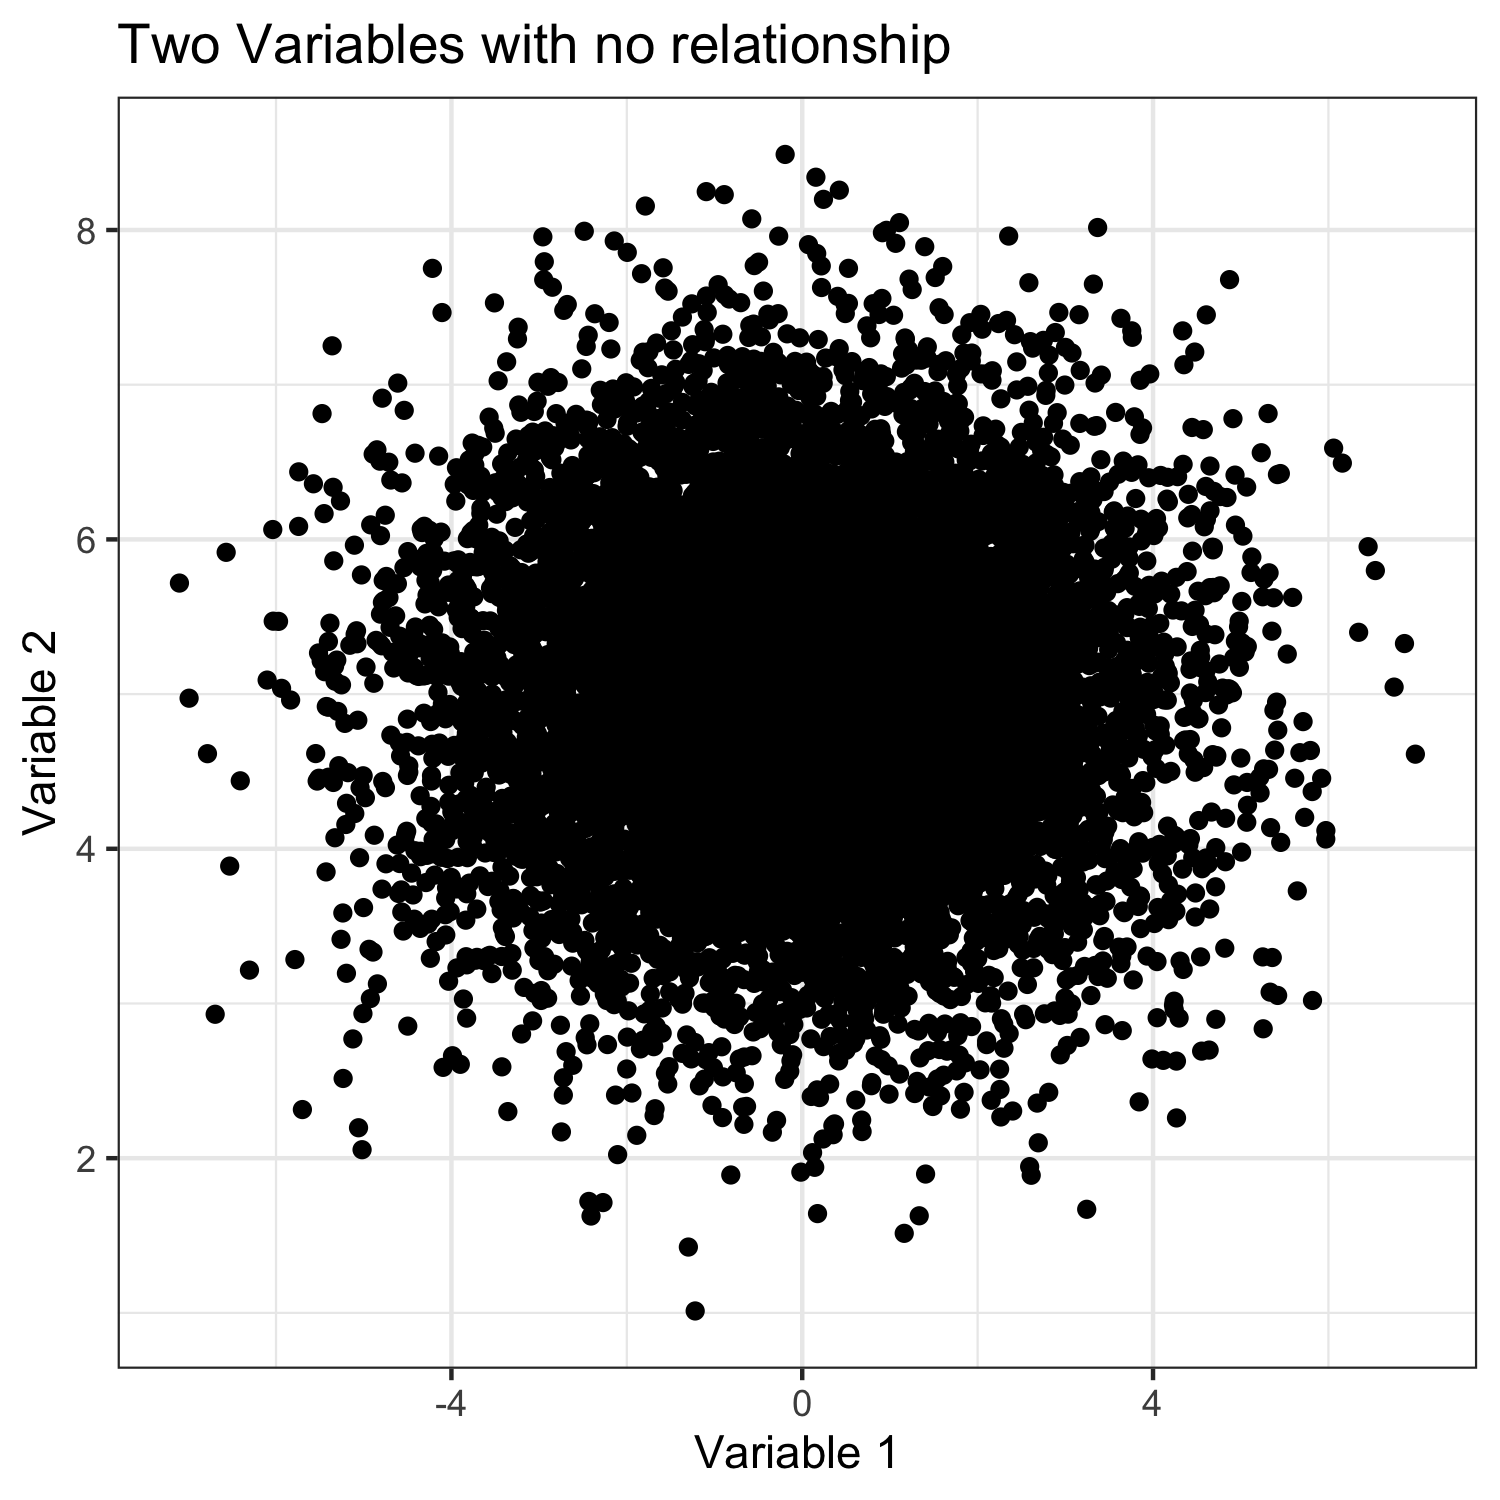
\includegraphics{/Users/timothyelder/Documents/plaintext_workshop/figures/war_fig.png}
\caption{There doesn't seem to be much of a relationship between these
two variables}\label{fig:example_fig}
}
\end{figure}

\begin{longtable}[]{@{}llll@{}}
\toprule()
& \textbf{Model 1} & \textbf{Model 2} & \textbf{Model 3} \\
\midrule()
\endhead
\textbf{(Intercept)} & -0.039 & -0.030 & 0.020 \\
& (0.072) & (0.068) & (0.059) \\
\textbf{biscuits} & 0.359*** & 0.327*** & 0.239*** \\
& (0.045) & (0.044) & (0.041) \\
\textbf{chips} & & 0.110** & 0.085** \\
& & (0.034) & (0.029) \\
\textbf{cheese} & & & 0.206*** \\
& & & (0.035) \\
\textbf{Deviance} & 49.369 & 44.521 & 32.481 \\
\textbf{N} & 100 & 100 & 100 \\
\bottomrule()
\end{longtable}

\hypertarget{conclusion}{%
\section{Conclusion}\label{conclusion}}

War? What is it good for?

\hypertarget{references}{%
\section{References}\label{references}}

\setlength{\parindent}{-0.2in}
\setlength{\leftskip}{0.2in}
\setlength{\parskip}{8pt}
\vspace*{-0.2in}

\noindent

\hypertarget{refs}{}
\begin{CSLReferences}{1}{0}
\leavevmode\vadjust pre{\hypertarget{ref-bennett_edward_1998}{}}%
Bennett, M. 1998.
{``\href{https://doi.org/10.1093/ehr/CXIII.452.580}{Edward {III}'s
{Entail} and the {Succession} to the {Crown}, 1376-1471}.''} \emph{The
English Historical Review} CXIII(452):580--609.

\leavevmode\vadjust pre{\hypertarget{ref-carpenter_wars_1997}{}}%
Carpenter, Christine. 1997. \emph{The {Wars} of the {Roses}: Politics
and the Constitution in {England}, c. 1437-1509}. {Cambridge ; New York,
NY, USA}: {Cambridge University Press}.

\leavevmode\vadjust pre{\hypertarget{ref-chrimes_henry_1999}{}}%
Chrimes, S. B. 1999. \emph{Henry {VII}}. {New Haven}: {Yale University
Press}.

\end{CSLReferences}

\end{document}